\chapter{Implementaci\'on}
\label{cap:implementacion}

\section{Desarrollo de la aplicación}
Dentro del campo de procesamiento de textos, el análisis de letras de canciones no es el más popular, sin embargo existen algunos trabajos que nos han servido de guía para establecer los límites y punto de comienzo de nuestro proyecto. Sin duda el proyecto existente que más se ajusta a nuestra primera idea es \href{https://medium.com/@alexing/data-data-b82201ec1cf4}{\textit{Data, data}}, que hace un estudio exhaustivo de las canciones del cantante Uruguayo Jorge Drexler, tanto de la letra como de la música.

Como hemos comentado en el Capítulo 2, nuestros objetivos son obtener los sentimientos que predominan en diferentes países, y comprobar si la hipótesis que hemos establecido indicando que el tema dominante en España es el amor.

\section{Creación del conjunto de datos}
Nuestro punto de partida son los datos que encontramos en varios datasets de Kaggle \footnote{\url{https://www.kaggle.com/mousehead/songlyrics }} \footnote{\url{https://www.kaggle.com/gyani95/380000-lyrics-from-metrolyrics}}. Cuyo formato, en el primer caso, es el que se aprecia en la Figura \ref{fig:dataset1}. Se componede 4 columnas, la primera contiene el nombre del grupo, la segunda el título de la canción, seguida en la siguiente columna de un link que unido a http://www.lyricsfreak.com/ nos redirige a una página donde encontramos más información de la canción, como el año de publicación entre otros, y por último la letra.
\begin{figure}
	\centering
	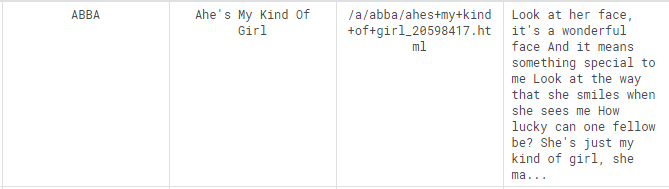
\includegraphics[width=0.7\linewidth]{Imagenes/dataset1}
	\caption{}
	\label{fig:dataset1}
\end{figure}
En el caso del segundo dataset, el formato es el que se aprecia en la Figura \ref{fig:dataset2}. En él encontramos el nombre del grupo, seguido del año de publicación de la canción, cuyo nombre aparece en la tercera columna, y finalmente la letra.
\begin{figure}
	\centering
	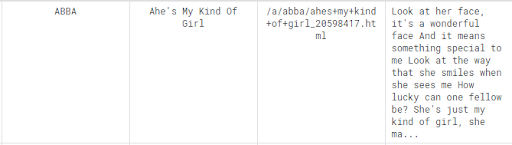
\includegraphics[width=0.7\linewidth]{Imagenes/dataset2}
	\caption{}
	\label{fig:dataset2}
\end{figure}

Un dato relevante en el desarrollo de ésta práctica del cual no disponemos a través de Kaggle es el país de procedencia de cada artista. Para obtenerlo utilizaremos técnicas de minería web para extraer dicha información a través de Wikipedia u otras fuentes. Una vez obtenida la información (país, autor, letras de sus canciones), limpiaremos los datos escogiendo sólo las palabras más relevantes, siendo éstas los verbos, sustantivos y adjetivos, eliminando artículos, conjunciones.

\section{Limpieza y preprocesamiento de los datos}
La limpieza de las letras es un paso crucial en el desarrollo de éste proyecto, puesto que muchas letras están compuestas de palabras que no aportan información relevante a la hora de realizar el análisis, como son los artículos, conjunciones, etc. Por ello, una vez obtenidos todos los datos, el paso siguiente será eliminar las llamadas \textit{stopwords} Figura \ref{fig:removeStopWords} , tanto del inglés como del castellano. Éste conjunto de palabras está compuesto por los tipos comentados anteriormente, es decir, palabras que no aportan información al análisis. Para ello, hemos desarrollado una función en R que, dado un texto, extrae únicamente las palabras que se encuentran en el diccionario, tanto en el de inglés como en el de castellano. Con ello buscamos evitar inconsistencias además de identificar y eliminar todos aquellos datos que aportarían ruido al análisis, como espacios extra o números.

\begin{figure}[h]
	\centering
	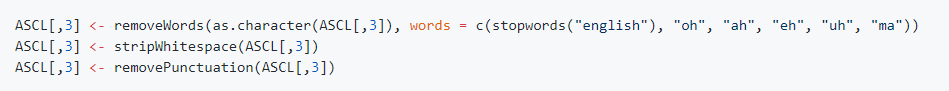
\includegraphics[width=1\linewidth]{Imagenes/removeStopWords}
	\caption{\textit Código en el que se retiran las llamadas "stopwords"}
	\label{fig:removeStopWords}
\end{figure}

El dataframe resultante contendrá, pues, 3 columnas indicando el grupo, la canción y las letras de cada canción. Figura \ref{fig:removeStopWords}

\begin{figure}[h]
	\centering
	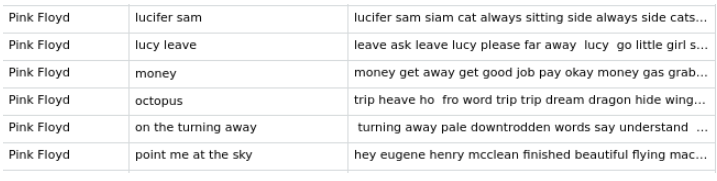
\includegraphics[width=1\linewidth]{Imagenes/datasetDataCleaning}
	\caption{\textit{DataFrame resultante del pre-procesamiento de datos}}
	\label{fig:datasetDataCleaning}
\end{figure}

Hemos tenido que eliminar los carácteres raros que no se encuentren en el diccionario en inglés (y también las palabras que los contienen) ya que no nos serán útiles para analizar el sentimiento de las canciones. Para ello utilizaremos funciones basadas en la librería  \textit{"qdapDictionaries"}. En este caso, como se puede ver en la figura \ref{fig:isWord}, la cual devolverá si la palabra introducida como parámetro está en inglés o español.

\begin{figure}[h]
	\centering
	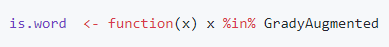
\includegraphics[width=0.8\linewidth]{Imagenes/isWord}
	\caption{\textit {Función usada en el proceso de eliminar carácteres raros y palabras que los contienen}}
	\label{fig:isWord}
\end{figure}

Crearemos un data frame en el que tendremos disponible la cantidad de canciones de cada grupo, junto al nombre del mismo. Figura \ref{fig:artistsDatframe}

\begin{figure}[h]
	\centering
	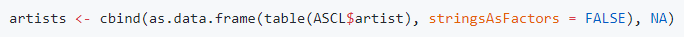
\includegraphics[width=0.9\linewidth]{Imagenes/artistsDatframe}
	\caption{\textit{Creación del data Frame con los artistas y la frecuencia de sus canciones}}
	\label{fig:artistsDatframe}
\end{figure}

Para facilitar el trabajo a la hora de identificar el nombre de los artistas, normalizaremos el nombre de los grupos para que tengan todos la misma forma. Figura \ref{fig:artistsStand}

\begin{figure}[h]
	\centering
	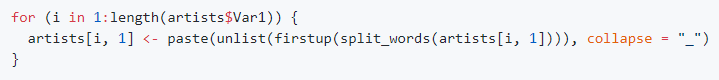
\includegraphics[width=0.9\linewidth]{Imagenes/artistsStand}
	\caption{Estandarizamos el nombre de los artistas}
	\label{fig:artistsStand}
\end{figure}



Como parte del preprocesamiento de los datos y con el fin de obtener una descripción más visual del set de datos obtenido, hemos realizado algunas pruebas. En primer lugar, hemos obtenido las palabras que aparecen en las canciones más conocidas del grupo Queen.

\begin{figure}[h]
	\centering
	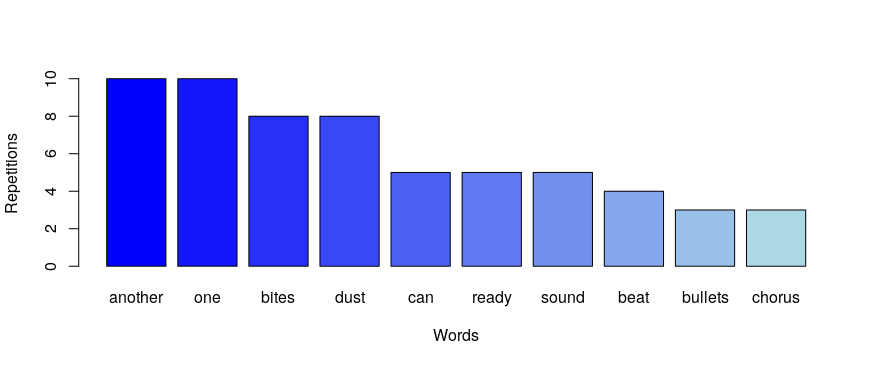
\includegraphics[width=0.7\linewidth]{Imagenes/AnotherOneBitesTheDust}
	\caption{\textit{Another One Bites the Dust} - Queen}
	\label{fig:AnotherOneBitesTheDust}
\end{figure}
\begin{figure}[!h]
	\centering
	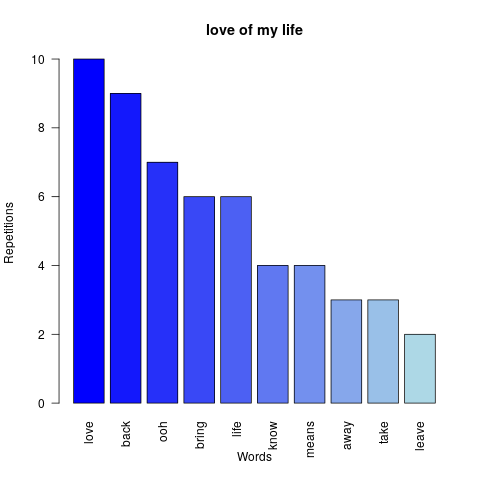
\includegraphics[width=0.7\linewidth]{Imagenes/loveofmylife}
	\caption{\textit{Love Of My life} - Queen}
	\label{fig:loveofmylife}
\end{figure}
\begin{figure}[!h]
	\centering
	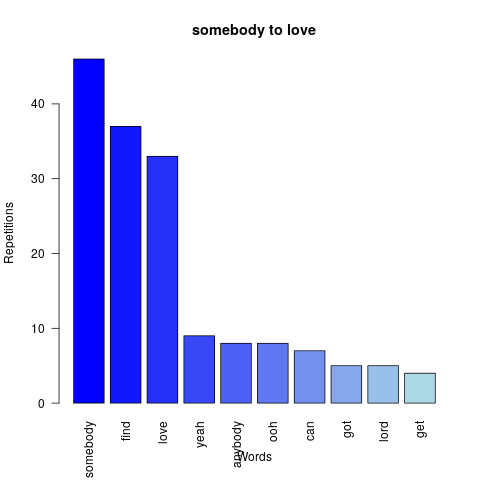
\includegraphics[width=0.7\linewidth]{Imagenes/somebodytolove}
	\caption{\textit{Somebody To Love} - Queen}
	\label{fig:sbtl}	
\end{figure}
\begin{figure}[!h]
	\centering
	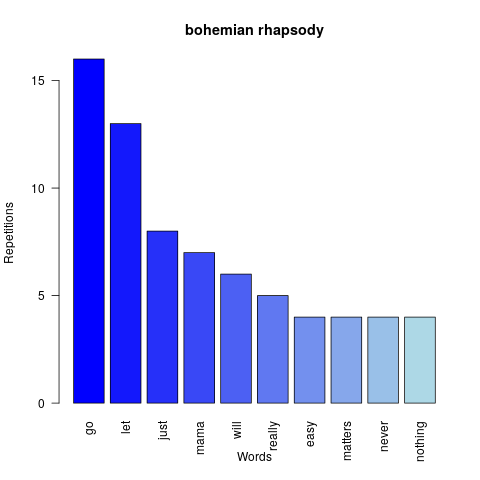
\includegraphics[width=0.7\linewidth]{Imagenes/bohemianrhapsody}
	\caption{\textit{Bohemian Rhapsody} - Queen}
	\label{fig:bohemianrhapsody}
\end{figure}
\begin{figure}[!h]
	\centering
	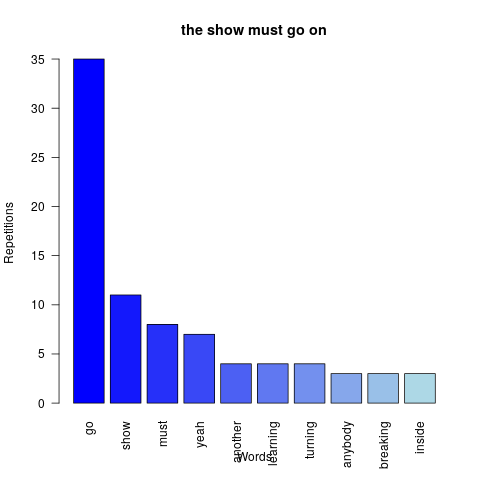
\includegraphics[width=0.7\linewidth]{Imagenes/theshowmustgoon}
	\caption{\textit{The Show must go on} - Queen}
	\label{fig:tsmgo}
\end{figure}




\begin{figure}[h]
	\centering
	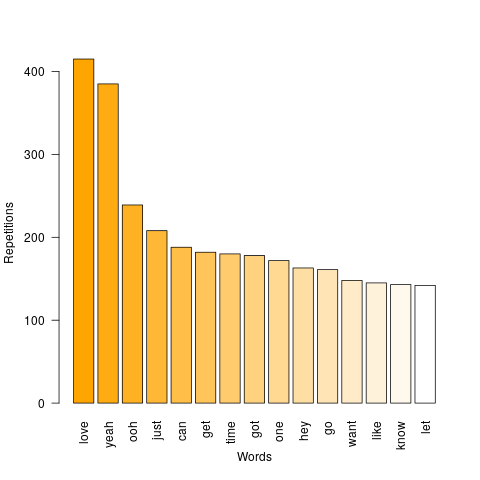
\includegraphics[width=0.7\linewidth]{Imagenes/queen_most_used_words}
	\caption{Most used words by Queen}
	\label{fig:queen_songs}
\end{figure}


Finalmente, tras estudiar los gráficos obtenidos y ver que tiene sentido que las palabras más utilizadas en dichas canciones son las que se muestran, procedemos a generalizar un poco más nuestra exploración, para ver cuales son las palabras más utilizadas por el grupo británico. Como se muestra en la figura \ref{fig:queen_songs}, la palabra \textit{amor} aparece más de 400 veces en las canciones de las que disponemos de dicha banda.


\section{Transformación de los datos}
Para poder trabajar de manera eficiente y general con los datos no es suficiente con una estructura que los contenga a todos, ya que en R concretamente podemos encontrar algunas que trabajan con tipos de datos heterogéneos. Si bien los datos en bruto comparten el tipo \textbf{character}, el conjunto cuenta con caracteres específicos no comunes en el lenguaje habitual además de variar entre mayúsculas y minúsculas. Este último detalle es vital ya que para el reconocimiento de palabras, tanto para su análisis como su limpieza, la homogeneidad de los datos será fundamental.

Tras trabajar con diferentes características homogéneas, concluimos que las letras de las canciones y sus títulos han de transformarse a minúsculas y el nombre de los artistas mantenerlo según la fuente para poder usarlo en búsquedas posteriores con técnicas de minería web.




\section{Elección de la tarea de minado adecuada}

Para conseguir extraer el sentimiento de las canciones utilizaremos diccionarios de sentimientos Figura \ref{fig:diccionariosentimientos}, en los cuales diferentes palabras tienen asignados uno o más sentimientos. Para ello elaboraremos diferentes funciones para determinar tanto el sentimiento de cada palabra, lo cual nos permitirá extraer el sentimiento general tanto del artista como del país al que pertenece.

También necesitaremos extraer el pais de origen de cada artista, para ello utilizaremos técnicas de minería web para extraer dicha información de Wikipedia.

\begin{figure}[h!]
	\centering
	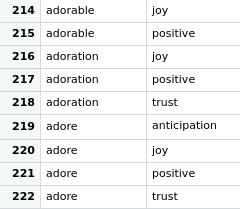
\includegraphics[width=0.6\linewidth]{Imagenes/diccionariosentimientos}
	\caption{Diccioanrio con los sentimientos}
	\label{fig:diccionariosentimientos}
\end{figure}

\section{Elección del algoritmo de minería de datos}

A la hora de decidir cómo afrontar la clasificación de sentimientos una de las opciones que barajamos fue usar el clustering para saber si podíamos agrupar el conjunto de datos en base al sentimieno predominante. 

Para ello aplicamos el método "K-Means" sobre el dataframe que veremos más adelante que agrupa los sentimientos de los países. Con tres clusters no nos aportó resultados relevantes. Después probamos con "DIANA" para dejar al algoritmo decidir, pero tampoco conseguimos gran cosa. Por ello decidimos afrontar el problema con la mentalidad de abarcar todo el dataset, para ello, en la siguiente sección explicaremos todos los pasos ejecutados.

\section{Aplicación del algoritmo elegido}

Para poder utilizar el diccionario de sentimientos primero necesitaremos descomponer las palabras que conforman las letras de las canciones, para ello utilizaremos la función de la Figura \ref{fig:get_existing_words}. 

\begin{figure}[h]
	\centering
	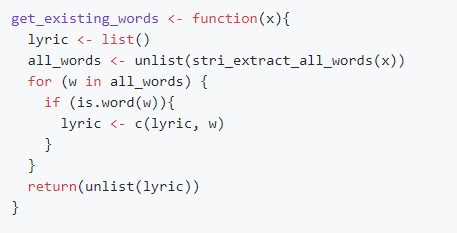
\includegraphics[width=0.7\linewidth]{Imagenes/get_existing_words}
	\caption{Función para extraer las palabras de las letras y existan en el diccionario }
	\label{fig:get_existing_words}
\end{figure}

Esta función iterará por todas las letras de las canciones y aquellas que estén presentes en el diccionario de sentimientos, las guardará. Como tiene que procesar cada palabra del total de 419887 canciones tiene un coste computacional muy elevado. Esto ha sido uno de los principales retos con los que nos hemos encontrado, ya que no podíamos ejecutar el algoritmo en cada iteración ya que tardaba muchas horas en realizarlo, para ello fuimos cogiendo pequeñas partes del data set a modo de pruebas para comprobar que los resultados eran satisfactorios.

El diccionario que usaremos está indicado en la Figura \ref{fig:word_sentiments}.


\begin{figure}[h]
	\centering
	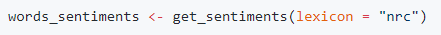
\includegraphics[width=0.7\linewidth]{Imagenes/word_sentiments}
	\caption{Diccionario que usaremos para la asignación de sentimientos}
	\label{fig:word_sentiments}
\end{figure}

 Ahora organizaremos las 419887 entradas por autores y tendremos un data frame resultante indicado en la figura \ref{fig:artistlyrics-dataframe}

\begin{figure}[h]
	\centering
	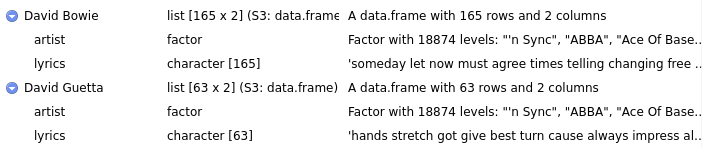
\includegraphics[width=0.9\linewidth]{Imagenes/artistlyrics-dataframe}
	\caption{Data frame resultante con los artistas agrupados con sus letras de las canciones}
	\label{fig:artistlyrics-dataframe}
\end{figure}

Con toda la información ordenada ya podemos asignar el sentimiento principal de cada artista con la función de la Figura \ref{fig:lista-sentimientos}. Esta función devolverá una lista de palabras, que serán los sentimientos, con la cual elaboraremos el data frame que asigna a cada artista el sentimiento principal tal y como se ve en la Figura \ref{fig:artista-sentimiento}.

Una vez tenemos listo el diccionario podemos asignar a cada palabra de las letras de cada artista los sentimientos que tiene asignados. Toda esta información la tendremos en un dataframe intermedio, el cual usaremos para obetener la frecuencia de todos los sentimientos y el que predomine lo asignaremos junto al autor en data frame principal Figura \ref{fig:artista-sentimiento}.

\begin{figure}[h]
	\centering
	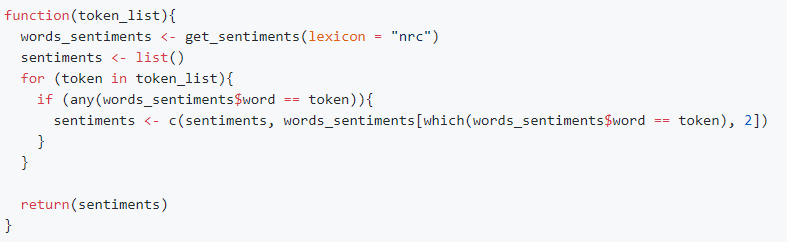
\includegraphics[width=\linewidth]{Imagenes/lista-sentimientos}
	\caption{Función para obtener los sentimientos de las palabras}
	\label{fig:lista-sentimientos}
\end{figure}

\begin{figure}[h]
	\centering
	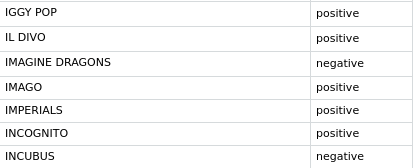
\includegraphics[width=0.7\linewidth]{Imagenes/artista-sentimiento}
	\caption{Tabla con el artista junto a su sentimiento predominante}
	\label{fig:artista-sentimiento}
\end{figure}


La parte final será pues, obtener el país correspondiente de cada artista, para ello hemos utilizado técnicas de minería web. Vamos a utilizar Wikipedia como fuente para obtener el pais correspondiente, para ello, como la URL puede estar en diferentes formatos tenemos que obtener las distintas formas tal y como se indica en la Figura \ref{fig:artists-wikipedia}. 

\begin{figure}[h]
	\centering
	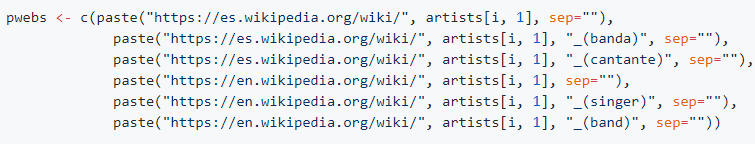
\includegraphics[width=0.7\linewidth]{Imagenes/artists-wikipedia}
	\caption{Diferentes formatos para obtener la URL}
	\label{fig:artists-wikipedia}
\end{figure}

Después, con la función de la Figura \ref{fig:link-exists} podremos saber cual de los links que hemos generado es el válido. 

\begin{figure}[h]
	\centering
	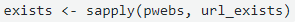
\includegraphics[width=0.7\linewidth]{Imagenes/link-exists}
	\caption{Comprueba cual de los links es válido}
	\label{fig:link-exists}
\end{figure}

Ese link, lo usaremos para finalmente obtener el artista, pero comprobaremos tanto la fuente en inglés como en español por si algún artista no tiene página en wikipedia en el otro idioma, de la forma mostrada en la Figura \ref{fig:asignar-oais}.

\begin{figure}[h]
	\centering
	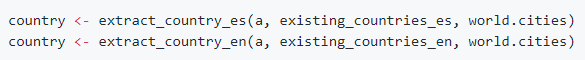
\includegraphics[width=0.7\linewidth]{Imagenes/asignar-oais}
	\caption{Extraer el pais adecuado de Wikipedia}
	\label{fig:asignar-oais}
\end{figure}

Con esta nueva información generamos dos data frames, el primero de la Figura \ref{fig:artistcountry} donde tendremos el artista junto con su cantidad de canciones y el pais correspondiente y el data set final de la Figura \ref{fig:sentimenttablebycountry} donde tenemos toda la información que necesitamos para inferir cual es el sentimiento general de cada país.

\begin{figure}[h]
	\centering
	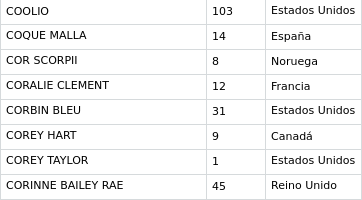
\includegraphics[width=0.7\linewidth]{Imagenes/artistcountry}
	\caption{Data frame con el artista, el número de canciones y el país}
	\label{fig:artistcountry}
\end{figure}

\begin{figure}[h]
	\centering
	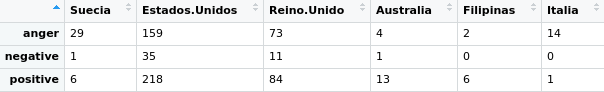
\includegraphics[width=0.7\linewidth]{Imagenes/sentimenttablebycountry}
	\caption{Data frame con los sentimientos de las canciones de cada país}
	\label{fig:sentimenttablebycountry}
\end{figure}
